\chapter{Technical Analysis}
The purpose of beam steering is to provide coverage in selected directions. This is enabled by having the main lobe of a radiation pattern of a directional antenna move to point towards the target of transmission and/or reception. Beam steering is purposeful for narrow directional beams. Beam steering can be performed using manual, mechanical or electronic with the main differences being method of implementation~\cite{ieee_beam_steering}~\cite{ieee_microchip_beam_steering}. This chapter explores the properties of antennas and beam steering methods, in order to understand antenna beam steering.

\section{Fundamentals of Antennas}
In order to develop a beam steering device for antennas it is necessary to understand antennas and their properties. Propagation, polarization, radiation characteristics are all properties of antennas that can vary based on the type of antenna.

\subsection{Propagation In Free Space}
Propagation of electromagnetic waves can be described with Maxwell's equations In differential form they are as follows~\cite[p. 1]{ant_beam_form}
\begin{equation}
    \begin{split}
        \nabla \times \textbf{E} & = - \frac{\partial }{\partial t} \textbf{B} \\
        \nabla \times \textbf{H} & = \textbf{J} + \frac{\partial }{\partial t} \textbf{D} \\
        \nabla \cdot \textbf{B} & = 0 \\
        \nabla \cdot \textbf{D} & = \rho
    \end{split}
\end{equation}

with \textbf{E} being the electric field with unit [\SI{}{\volt\per\meter}], \textbf{B} being induction [\SI{}{\tesla}], \textbf{H} is magnetic field [\SI{}{\ampere\per\meter}], \textbf{D} being dielectric displacement [\SI{}{\ampere\second\per\meter\squared}], \textbf{J} being the current density [\SI{}{\ampere\per\meter\squared}] and $\rho$ being electric charge density [\SI{}{\coulomb\per\meter\cubed}].

The electric field and the magnetic field are connected; the electric field is created by the magnetic field and vice versa. The electric field and the magnetic field in the spherical coordinate system $\left(r, \theta, \phi, t\right)$ are illustrated on figure \ref{fig:em_field} below.
\begin{figure}[H]
    \centering
    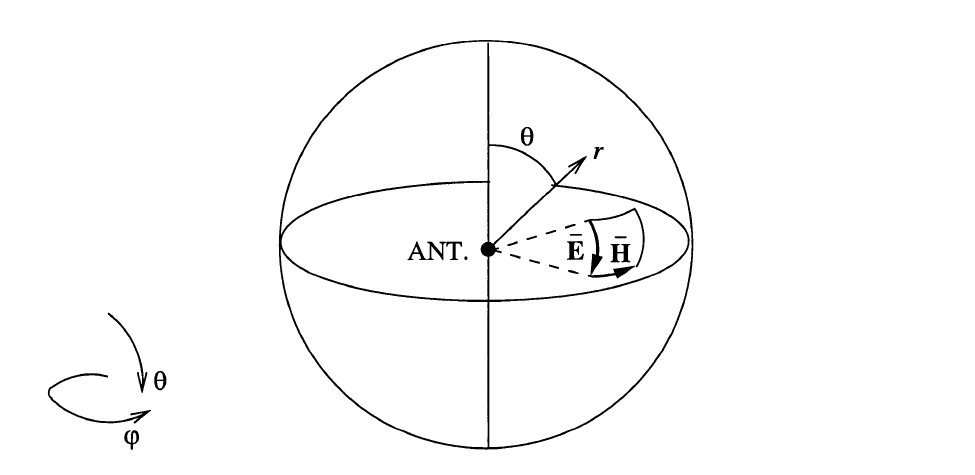
\includegraphics[width=0.6\textwidth]{figures/em_polar_coordinates.png}
    \caption{Electromagnetic propagation in the far field range around a small elemental antenna oriented along the z-axis visualised in the spherical coordinate system~\cite[p. 58]{maxwell_theory}.} \label{fig:em_field}
\end{figure}

As visualised on figure \ref{fig:em_field} the electric field only depends on the $\theta$-component and the magnetic field only on the $\phi$-component when in the far field. The vector \textbf{r} is direction of the observation point. The length of \textbf{r} is the distance to the observation point ie. distance between transmitting and receiving point~\cite[p. 59]{maxwell_theory}.

The Poynting vector describes the power density and direction of the electromagnetic flux and is the cross product of the electric and magnetic field 
\begin{equation}
    \textbf{S} = \textbf{E} \times \textbf{H}
    \tagaddtext{[\si{\watt\per\meter\squared}]}
\end{equation}
which points in the same direction as the wave propagation~\cite[p. 3]{ant_beam_form}. 

\subsubsection{Multipath propagation}
the signal that reaches the receiving antenna can have travelled other paths than the direct line-of-sight path from the transmitter. This is because electromagnetic waves can reflect on surrounding surfaces, be changed by condition of the transmission medium or be Doppler shifted due to movement of the receiver, transmitter or other objects. The received signal is a summation of all input signals regardless of phase angles, phase shifts or directions and therefore the received signal might be distorted~\cite[pp. 1-2]{itu_multipath}. 

%\subsubsection{Aliasing} \label{sss:aliasing}
%\to do[inline, color=red]{write about this}
%To prevent aliasing there must be a certain distance between the test device and the transmitting device, or in case of reflection measurement, half this length. The alias-free range is calculated as
%\begin{equation}
%    Range = \frac{1}{\Delta f} V_f c 
%    \tagaddtext{[\si{\meter}]}
%\end{equation}
%where $\Delta f$ is frequency step size, $V_f$ is the velocity factor in the transmission line which is $1$ for free space and c is the speed of light (\SI{300E6}{\meter\per\second}). The frequency step size is equal to the measured frequency span divided by the number of discrete points in the span and is therefore dependent on the settings made on the network analyzer~\cite[p. 27]{ks_td_analysis}. 

\subsection{Polarization} \label{ss:polarization}
Polarization describes the classification of the plane propagated wave, which is an electromagnetic wave that propagates with constant velocity in a specific direction. The direction of the propagation of the electromagnetic wave is always perpendicular to the direction of the electric field \textbf{E} and both are perpendicular to the direction of the magnetic field \textbf{H}. If the direction of the electric field is constant with time and position, the polarization of the propagated wave is classified as linear. If the direction of the electric field changes by rotating uniformly around the axis of the propagated wave, the wave has circular polarization. The polarization of the receiving and transmitting antennas affects how the signal is detected. The signal is best received when the polarization of the receiver is the same as the polarization for the transmitter. Mismatch in polarization will result in less received power or more noise in the signal~\cite[p. 82-84]{direct_energy}. 

Different antenna designs have different radiation patterns and polarization. Table \ref{tab:antenna_types} lists a number of different antenna designs and their polarization
\begin{table}[H]
    \centering
    \begin{tabular}{l|l} 
        \textbf{Type} & \textbf{Polarization} \\
        \hline
        \hline
        Isotropic antenna & \\
        Dipole antenna & Linear \\
        Patch antenna & Linear, circular \\
        Horn antenna & Linear, cicular \\
        Helical antenna & Circular \\
    \end{tabular}
    \caption{Table showing polarization of some typical antenna designs~\cite[p. 11]{ant_beam_form}.}
    \label{tab:antenna_types}
\end{table}

\subsection{Radiation Characteristics} \label{ss:rad_char}
Electromagnetic waves propagate away from the source. Depending on the distance from the source, the electromagnetic waves can be found in the near field or the far field. The far field is mathematically described as the distance $r>R_2$, with $R_2$ defined as~\cite[p. 4]{ant_beam_form}
\begin{equation} \label{eq:far_field}
    R_2 = \frac{2 D^2}{\lambda}
    \tagaddtext{[\si{\meter}]}
\end{equation}

with $D$ being the largest dimension of the antenna or antenna array and $\lambda$ being the wavelength of the carrier frequency.

The radiation characteristics of an antenna can be described by the directivity, which is defined as the ratio of the maximum power density $S\left( \theta, \phi \right)_{max}$ radiated to the average power density $S\left( \theta, \phi \right)_{avg}$ radiated by an antenna. The directivity is unitless~\cite[p. 63]{direct_energy}. An isotropic antenna is a theoretical antenna which radiates homogeneously in all directions, meaning that the magnitude of the power density vector \textbf{S} at a distance vector \textbf{r} is constant~\cite[p. 11]{ant_beam_form}
\begin{equation} \label{eq:isotropic_radiation}
    D_{iso}\left( \theta, \phi \right) = \left| \frac{S\left( \theta, \phi \right)_{max}}{S\left( \theta, \phi \right)_{avg}} \right|=1
\end{equation}

It is this theoretical isotropic radiator that the gain of antennas are in respect to. The directivity does not depend on the distance, $r$, in the far field, meaning that at the receiver, the relation $r \gg  R_2$ is assumed. The directivity can then be described by~\cite[p. 10]{ant_beam_form}
\begin{equation} \label{eq:directivity1}
    D \left( \theta, \phi \right) = \frac{S\left( \theta, \phi \right)_{max}}{S\left( \theta, \phi \right)_{avg}}
\end{equation}

The total radiated power $P_{r}$ is found by the surface integral of the power density. Assuming a spherical surface, the total radiated power is described as~\cite[p. 1-9]{ant_eng_hk}
\begin{equation} \label{eq:surface_integral}
    P_{r} = \int_{0}^{2 \pi} \int_{0}^{\pi} S\left( \theta, \phi \right) r^2 \sin \theta \, d\theta \, d\phi
    \tagaddtext{[\si{\watt}]}
\end{equation}
The average radiated power over every direction in the sphere is given by~\cite[p. 1-9]{ant_eng_hk}
\begin{equation} \label{eq:average_power}
    P_{avg} = \frac{P_{r}}{4 \pi r^2}
    \tagaddtext{[\si{\watt\per\meter\squared}]}
\end{equation}
Replacing the average power density $S\left( \theta, \phi \right)_{avg}$ in equation \ref{eq:directivity1} with the average radiated power, the directivity of an antenna $D \left(\theta, \phi \right)$ can be defined as~\cite[p. 10]{ant_beam_form}
\begin{equation} \label{eq:directivity}
    D\left(\theta, \phi\right) = 4 \pi r^2 \frac{S \left(\theta, \phi\right)_{max}}{P_{r}}
\end{equation}

with $S\left(\theta, \phi\right)_{max}$ being the maximum power density and $P_{r}$ being the total radiated power of the antenna.

The power of the source $P_{s,t}$ to a transmitting antenna might not equal the radiated power $P_{r,t}$ due to power loss $p_{l,t}$. Power loss can happen because of reflection loss in the input medium, conductor loss and dielectric loss. The efficiency of the transmitting antenna $\eta$ is described as the ratio of the radiated power to the sourced power 
\begin{equation} \label{eq:antenna_efficiency}
    \eta = \frac{P_{r,t}}{P_{s,t}} = \frac{P_{r,t}}{P_{r,t}+P_{l,t}}
\end{equation}

The gain $G \left( \theta, \phi \right)$ of the antenna is the effective directivity, meaning how well the receiving or transmitting antenna is able to convert either electromagnetic waves or power into the other. The gain of a transmitting antenna can be calculated as~\cite[p. 10]{ant_beam_form}
\begin{equation} \label{eq:gain}
    G_t \left( \theta, \phi \right) = \eta  D_t \left(\theta, \phi\right) = 4 \pi r^2 \frac{S \left(\theta, \phi\right)_{max}}{P_{s,t}}
\end{equation}

or expressed in decibel with respect to the isotropic radiator~\cite[p. 10]{ant_beam_form}~\cite[pp. 1.8-1.10]{ant_eng_hk}.
\begin{equation} \label{eq:gain_dbi}
    G_{dBi} = 10 \log_{10}\left(G\right)
    \tagaddtext{[\si{\decibel}]}
\end{equation}

\subsection{Friis' Transmission Equation} \label{ss:friis}
The Friis transmission equation explains how the received power at a receiver is related to the power of the transmitter. The receiver antenna receives energy from the transmitting antenna and the effectiveness of this is described as the effective area $A_r\left( \theta, \phi \right)$ assuming that the antenna is placed in the origin of the spherical coordinate system. If the antenna has the property of reciprocity, the effective area and the gain of the receiver antenna is related by~\cite[p. 1.10]{ant_eng_hk}
\begin{equation} \label{eq:effectivate_area}
    A_r \left( \theta, \phi \right) = \frac{\lambda^2}{4 \pi} G_r \left( \theta, \phi \right)
    \tagaddtext{[\si{\meter\squared}]}
\end{equation}

If the gain of the transmitting antenna, $G_t$, is in the direction of the receiver antenna then the angular dependencies of the antenna properties can be surpressed. The power of the receiving antenna is equal to the power density $S \left(\theta, \phi\right)$ multiplied by the effective area of the receiver antenna $A_r$, expressed as
\begin{equation} \label{eq:receiver_power}
    P_r = S_t A_r
    \tagaddtext{[\si{\watt}]}
\end{equation} 

As previously mentioned the directivity of an antenna does not depend on the distance $r$ from the antenna, and likewise so with the power density $S_t$, so the value of $S_t$ is equal regardless of the distance from the antenna in the far field with respects to the angular dependencies. Substituting $S_t$ and $A_r$ in equation \ref{eq:receiver_power} for $S_t$ isolated in equation \ref{eq:gain} and $A_r$ from equation \ref{eq:effectivate_area} yields
\begin{equation} \label{eq:friis}
    \begin{split}
        P_r & = \frac{G_t P_t}{4 \pi r^2} \frac{\lambda^2 G_r}{4 \pi} \\
        & = G_t  G_r P_t \left( \frac{\lambda}{4 \pi r} \right)^2
        \tagaddtext{[\si{\watt}]}
    \end{split}
\end{equation} 

This is referred to as Friis' transmission equation~\cite[pp. 1.10-1.11]{ant_eng_hk}. The radiation characteristics of an antenna in the far field is called the antenna radiation pattern and will look different depending on the design of the antenna. The radiatation pattern is dependent on the anglular properties $\theta$ and $\phi$ and is usually visualised in a plane parallel to the electric field and called an \textbf{E} plane pattern or elevation plane pattern, or parallel to the magnetic field and called a \textbf{H} plane pattern or Azimuth plane pattern~\cite[p. 79-80]{direct_energy}\cite[p. 13-14]{ant_beam_form}.

\subsection{S-Parameters} \label{ss:s_params}
S-parameters are used to describe the input and output relationship of a system's ports at microwave frequency~\cite{s_params}. S-parameters are used because voltages and currents can be difficult to measure directly in the microwave frequency spectrum. S-parameters describe a network in waves instead of voltages and currents~\cite{ming_notes}. S-parameters can be used to describe an \textit{n}-port, $n\geq1$, system and are dependent on frequency~\cite{s_params}. Some typical systems are one-port and two-port systems, visualised in figures \ref{fig:1p_sys} and \ref{fig:2p_sys}.
\begin{figure}[H]
    \begin{minipage}{0.45\textwidth}
        \centering
        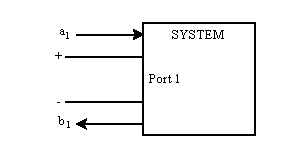
\includegraphics[width=0.7\textwidth]{figures/1p_system.pdf} % first figure itself
        \caption{One-port system.} \label{fig:1p_sys}
    \end{minipage}\hfill
    \begin{minipage}{0.45\textwidth}
        \centering
        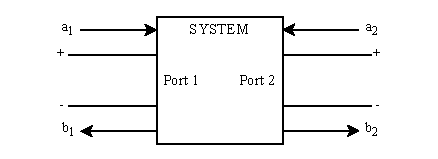
\includegraphics[width=0.9\textwidth]{figures/2p_system.pdf} % second figure itself
        \caption{Two-port system.} \label{fig:2p_sys}
    \end{minipage}
\end{figure}

The parameters \textit{a} and \textit{b} represent the waves flowing in and out of the system and they represent linear combinations of the voltages and currents at the ports~\cite{ming_notes}.Looking at a two-port system, such as a system with a receiver antenna and transmitter antenna, the S-parameter matrix looks as follows:
\begin{align} \label{eq:s_matrix}
    \begin{bmatrix} b_1 \\ b_2 \end{bmatrix} = 
    \begin{bmatrix} s_{11} & s_{12} \\ s_{21} & s_{22} \\ \end{bmatrix} \begin{bmatrix} a_1 \\ a_2 \end{bmatrix}
\end{align}

The S-parameters represent different information about the system as table \ref{tab:s_params} illustrates.
\begin{table}[H]
    \centering
    \begin{tabular}{p{0.15\textwidth}|p{0.6\textwidth}}
        \textbf{Parameter} & \textbf{Description} \\
        \hline
        \hline
        $S_{11}$ & $S_{11}=\frac{b_1}{a_1}$. Forward reflection coefficient. Describes the input return loss $\Gamma$ i.e. what is reflected from the port rather than radiated or absorbed. \\
        $S_{12}$ & $S_{12}=\frac{b_1}{a_2}$. Reverse transmission coefficient i.e. how much is transmitted from port 2 to port 1. \\
        $S_{21}$ & $S_{21}=\frac{b_2}{a_1}$. The forward transmission coefficient i.e. how much is transmitted from port 1 to port 2. \\
        $S_{22}$ & $S_{22}=\frac{b_2}{a_2}$. Reverse reflection coefficient i.e. output matching. \\
    \end{tabular}
    \caption{Explanation of S-parameters~\cite{s_params}.}
    \label{tab:s_params}
\end{table}

Ideally, an electrical load is designed to have the least possible input return loss. This means the power transfer is maximised or the signal reflection is minimised, depending on the use case.Minimal reflection is achieved when the complex output impedance is equal to the complex input impedance and maximum power transfer is achieved when the complex output impedance is equal to the complex conjugate of the input impedance. If the input impedance of an electrical load is denoted $Z_L$ and the characteristic output impedance of a signal source is denoted $Z_0$~\cite{s_params}\cite{ming_notes}, the return loss can be calculated as
\begin{equation} \label{return_loss}
    \Gamma = \frac{Z_L-Z_0}{Z_L+Z_0}
\end{equation}

Using the reflection coefficient the output flow at port one of a system is equal to $b_1=\Gamma a_1$~\cite{ming_notes}. $S_{11}$ and the reflection coefficient $\Gamma$ are related as follows:
\begin{equation}
    S_{11} = 20 \log_{10}\left(\left|\Gamma\right|\right)
    \tagaddtext{[\si{\decibel}]}
\end{equation}

\section{Antenna Designs} \label{ss:antenna_design}
The design of the antenna affects the radiation characteristics, the bandwidth and the range of frequencies at which the antenna is able to transmit or receive at~\cite[p. 76]{direct_energy}. Bandwidth is the range of frequencies where the antenna is expected to operate in the wanted manner. There are several criterias that can be used to decide on the bandwidth for an antenna, for example the range where the reflection coefficient is less than a specified value or when the polarization fits a certain shape. The antenna design can also be designed to operate with a given bandwidth. The radiation pattern of an antenna varies with the frequency but the general shape is primarily decided by the design of the antenna~\cite{bandwidth}. The antenna types described in table \ref{tab:antenna_types} are some typical design types along with the isotropic antenna which is a theoretical antenna~\cite[p. 11]{ant_beam_form}.

A center-driven dipole antenna is two wires or rods pointing at the opposite direction of each other, for example towards positive and negative \textit{z} in the spherical coordinate system. In the Azimuth plane the radiation pattern is a circle centered at the centre of the dipole antenna, whereas in the elevation plane, the radiation pattern is two ears extending from the centre to either side (see figure \ref{fig:dipole_1})~\cite[pp. 12-14]{ant_beam_form}. The figure \ref{fig:dipole_1} shows a typical radiation pattern for a one-wavelength dipole antenna. As seen, the dipole antenna has a uniform pattern. Increasing the length of the dipole can increase the directiveness. However, the length also affects the input impedance. The dipole antenna will always have linear polarization~\cite{dipole}. 
\begin{figure}[H]
    \begin{minipage}{0.45\textwidth}
        \centering
        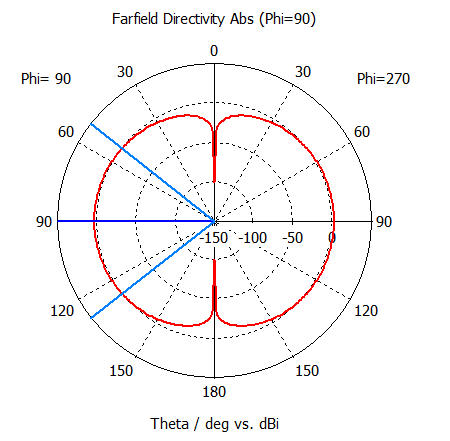
\includegraphics[width=0.9\textwidth]{figures/farfield (f=2.4) dipole.png} % first figure itself
    \end{minipage}\hfill
    \begin{minipage}{0.45\textwidth}
        \centering
        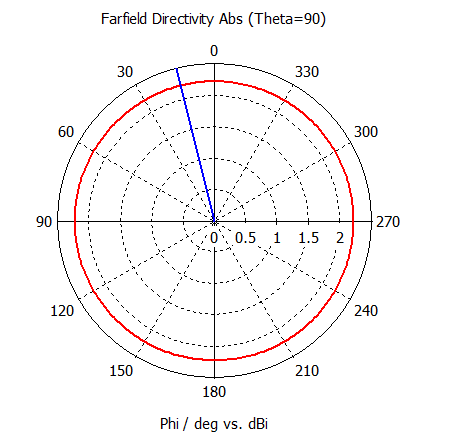
\includegraphics[width=0.9\textwidth]{figures/farfield (f=2.4) dipole_1.png} % second figure itself
    \end{minipage}
    \caption{Dipole antenna radiation pattern. Figures generated with \textit{CST Studio} dipole antenna example ($f=\SI{2.4}{\giga\hertz}$). The distance between the rods is \SI{3.12}{\milli\meter}, the radius is \SI{0.42}{\milli\meter}, the length is one half-wavelength or \SI{62.5}{\milli\meter}.}
    \label{fig:dipole_1}
\end{figure}

A patch antenna is in its simplest form a piece of metal on top of a grounded surface. The metal can have different shape and size to accomodate different operating frequencies, bandwidths and gains. The feeding of the patch can also affect the antenna parameters such as the impedance match. The patch antenna is usually only used for microwave applications, because the flatness of the antenna allows it to fit into narrow areas, where the patch size must also be small. The operating frequencies depend on the size of the patch and vice versa. The patch antenna has lower efficiency than many other antenna design types, and a small bandwidth~\cite[p. 7.3]{ant_eng_hk}. The radiatation pattern depends, as in all cases, on the design of the patch, and can have a large variety of shape~\cite[p. 7.1-7.5]{ant_eng_hk}. An example can be seen in figure \ref{fig:patch_1}.
\begin{figure}[H]
    \begin{minipage}{0.45\textwidth}
        \centering
        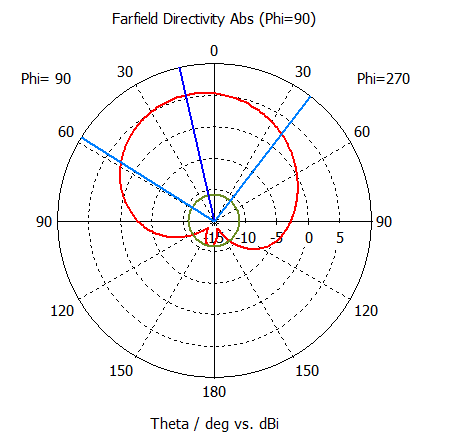
\includegraphics[width=0.9\textwidth]{figures/farfield (f=2.4) patch.png} % first figure itself
    \end{minipage}\hfill
    \begin{minipage}{0.45\textwidth}
        \centering
        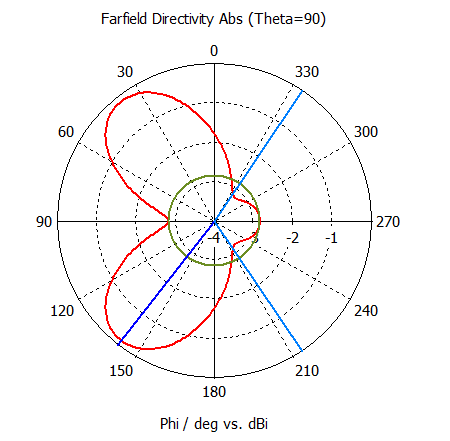
\includegraphics[width=0.9\textwidth]{figures/farfield (f=2.4) patch_1.png} % second figure itself
    \end{minipage}
    \caption{Patch antenna radiation pattern. Figures generated with \textit{CST Studio} ($f=\SI{2.4}{\giga\hertz}$). The dimensions are width \SI{47}{\milli\meter}, height \SI{30.2}{\milli\meter}, inset width \SI{1.5}{\milli\meter}, inset height \SI{7.16}{\milli\meter}, dielectric height \SI{1.5}{\milli\meter}, substrate width and height \SI{80}{\milli\meter} and transmission line length \SI{2.98}{\milli\meter}.}
    \label{fig:patch_1}
\end{figure}

Horn antennas come in many shapes and sizes which affect the radiation pattern and gain but common amongst the different designs is high beam directivity. A pyramidal, rectangular horn antenna is a common horn antenna, and has a fan-shaped radiation pattern. The gain can be calculated by knowing its dimensions and the beamwidth of the fan can be changed by the varying the aperture dimensions. Horn antennas can be designed to cover both wide and narrow bandwidths, linear or circular polarization or to have a certain gain. Horn antennas are regarded as being able to fulfill many different applications~\cite[p. 14.1-14.3]{ant_eng_hk}.  
\begin{figure}[H]
    \begin{minipage}{0.45\textwidth}
        \centering
        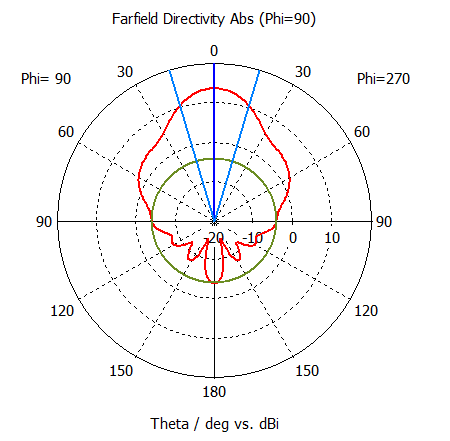
\includegraphics[width=0.9\textwidth]{figures/farfield (f=2.4) horn.png} % first figure itself
    \end{minipage}\hfill
    \begin{minipage}{0.45\textwidth}
        \centering
        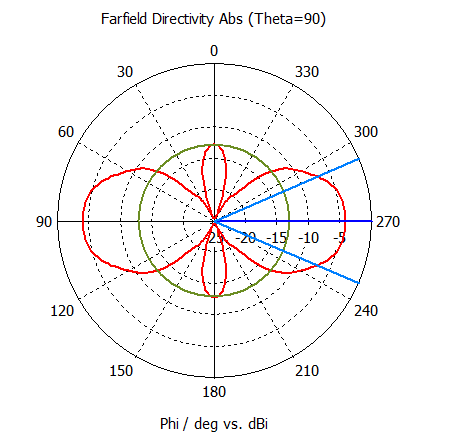
\includegraphics[width=0.9\textwidth]{figures/farfield (f=2.4) horn_1.png} % second figure itself
    \end{minipage}
    \caption{Horn antenna radiation pattern. Figures generated with \textit{CST Studio} horn antenna example ($f=\SI{2.4}{\giga\hertz}$). The antenna has a aperture width of \SI{288}{\milli\meter}, aperture height of \SI{211}{\milli\meter}, flare length \SI{111}{\milli\meter}, metal thickness \SI{0.62}{\milli\meter}, waveguide height \SI{49}{\milli\meter}, waveguide length \SI{125}{\milli\meter} and waveguide width \SI{98}{\milli\meter}.}
    \label{fig:horn_1}
\end{figure}

A helical antenna is one or several conductors in a helical shape connected to a ground plane and can be configured in many modes, the typical being \textit{normal} or \textit{axial} mode. Normal mode is achieved when the diameter of the helix is smaller than a wavelength and axial mode is when the circumference is close to the wavelength. A helix antenna has circular polarization in either right-hand or left-hand direction. A helix antenna has a wide spectrum for which impedance characteristics can be matched~\cite[p. 12.2]{ant_eng_hk}.
\begin{figure}[H]
    \begin{minipage}{0.45\textwidth}
        \centering
        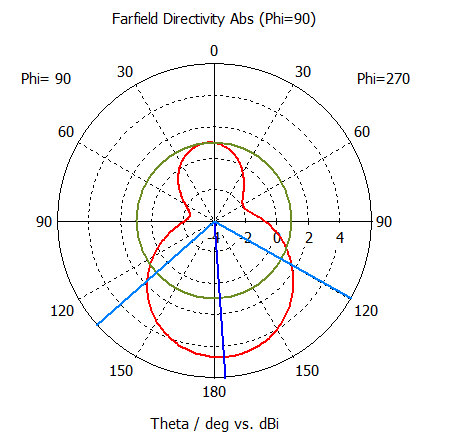
\includegraphics[width=0.9\textwidth]{figures/farfield (f=2.4) helical.png} % first figure itself
    \end{minipage}\hfill
    \begin{minipage}{0.45\textwidth}
        \centering
        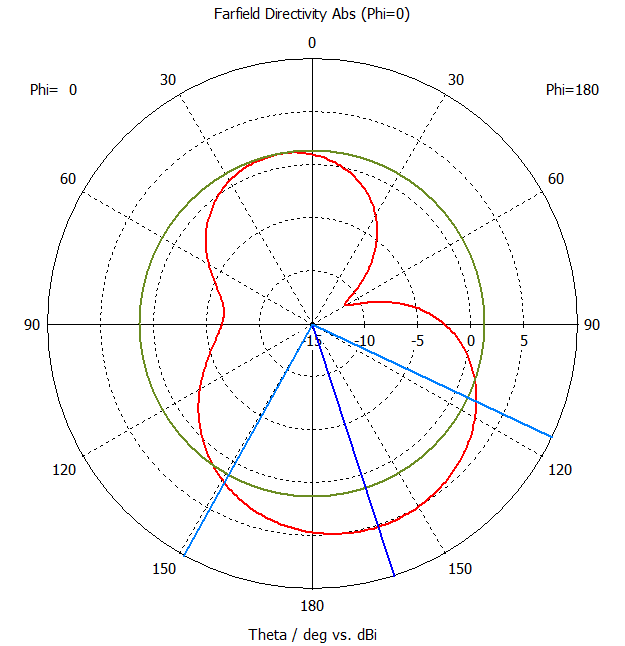
\includegraphics[width=0.9\textwidth]{figures/farfield (f=2.4) helical_1.png} % second figure itself
    \end{minipage}
    \caption{Helical antenna radiation pattern. Figures generated with \textit{CST Studio} ($f=\SI{2.4}{\giga\hertz}$). The coil dimensions are: height \SI{67}{\milli\meter}, number of turns \SI{9}{}, clockwise orientation, segmentation angle $\phi=\SI{14}{\degree}$, major and minor radius \SI{4.77}{\milli\meter}.}
    \label{fig:helical_1}
\end{figure}

\section{Beam Steering Methods}
Although the design of the antenna or antenna arrays decide the pattern of radiation, it is possible to modify this pattern or the direction of the pattern to achieve different directivities for other applications. The beam of the antenna can be steered in different directions for example, in order to cover a larger physical area with a single or few antennas or to focus a beam in a certain direction. Beam steering can be done manually, mechanically or electrically.

\subsection{Electrical Steering}
Electrical beam steering is the conventional steering method which builds upon beam forming methods. Beam forming means forming a single beam from a phased antenna array and controlling the shape and direction of this beam. Electrical beam steering does therefore not require changing the hardware or the setup but instead requires some form of control mechanism. Looking at a array of antennas, each element can be fed seperately to be able to change the phase and magnitude of each antenna element. Otherwise, if the antennas are fed with the same signal, the electromagnetic waves will combine and strengthen in the direction perpendicular to the antenna plane~\cite{beamsteering}.

\subsection{Manual and Mechanical Steering}
Manual or mechanical steering differs from electrical steering in that it is not the beam that is steered but the antenna as a whole. For mechanical steering the antenna can be mounted on a rotating platform or arm that is controlled by a motor. There are several motor types that can rotate a platform or arm holding an antenna, for example a step motor or a servo motor. 

A step motor has a rotor with two segments seperated by a permanent magnet. The rotor segments have teeth which become poles of opposite polarity when the permanent magnet is axially magnetized. The rotor segments are also always skewed so that the teeth of one segment aligns with the gap between the teeth of the other rotor segment. The number of teeth determines the number of position steps around the center axis. The stator then generates a rotating magnetic field when the windings in the stator are supplied with current. The driver of the step motor controls the input current with PWM signals. The step motor usually works in an open loop configuration because of the design does not require feedback, however, overloading the motor might cause loss of synchronisation~\cite{servo_step}. Figure \ref{fig:open_loop} below shows a block diagram of an open loop configuration.
\begin{figure}[H]
    \centering
    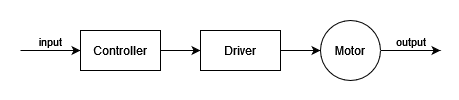
\includegraphics[width=0.6\textwidth]{figures/open-loop.png}
    \caption{Open loop motor control block diagram~\cite{loop}.} \label{fig:open_loop}
\end{figure}

Mathematically, the open loop configuration can be described by the open loop transfer function without feedback
\begin{equation}
    \frac{Y(s)}{R(s)} = G(s)D(s)M(s)
\end{equation}

Servo motors use a radially magnetized rotor, which means the number of poles determines the number of position steps around the center axis. This usually mean that a servo motor has less available positions than a step motor. The servo motor works like the step motor but an encoder is also used in the motor to give feedback to minimize error in the position~\cite{servo_step}. The servo motor loop configuration can be seen on figure \ref{fig:closed_loop} 

\begin{figure}[H]
    \centering
    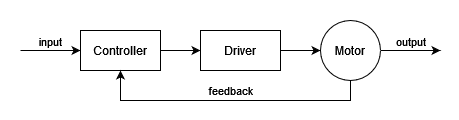
\includegraphics[width=0.6\textwidth]{figures/closed-loop.png}
    \caption{Closed loop motor control block diagram~\cite{loop}.} \label{fig:closed_loop}
\end{figure}

Mathematically, the closed loop configuration, with feedback denoted $H(s)$, can be described by the closed loop transfer function
\begin{equation}
    \frac{Y(s)}{R(s)} = \frac{G(s)D(s)M(s)}{1+G(s)D(s)M(s)H(s)}
\end{equation}

The step and servo motor differ when it comes to the relationship between the speed and the torque characteristics. The step motor has high torque at low speeds which drops significantly as the speed increases. The servo motor has a flat torque up until high speeds. Usually, the step motor is most ideal for applications where discrete position accuracy and fast responsiveness is valued whereas the servo motor is most ideal in applications with high or varying loads~\cite{servo_step}.